\documentclass[Journal,letterpaper,InsideFigs]{ascelike-new}
% Submit to ASCE Journal of Pipeline Engineering and Practice
\usepackage[utf8]{inputenc}
\usepackage[T1]{fontenc}
\usepackage{booktabs}
\usepackage{lmodern}
\usepackage{graphicx}
\usepackage[figurename=Fig.,labelfont=bf,labelsep=period]{caption}
\usepackage{subcaption}
\usepackage{amsmath}
\usepackage{amsfonts}
\usepackage{amssymb}
\usepackage{amsbsy}
\usepackage{newtxtext,newtxmath}
\usepackage[colorlinks=true,citecolor=red,linkcolor=black]{hyperref}
\usepackage{cleveref}
%
% Please add the first author's last name here for the footer:
%\NameTag{Kumar, \today}
%
\begin{document}

% You will need to make the title all-caps
\title{Conductive and convective heat transfer in inductive heating of subsea buried pipelines}

\author[1]{Krishna Kumar}
\author[2]{Chadi El Mohtar}
\author[2]{Robert Gilbert}

\affil[1]{Civil, Architectural and Environmental Engineering, University of Texas at Austin. Email: krishnak@utexas.edu}
\affil[2]{Civil, Architectural and Environmental Engineering, University of Texas at Austin}

\maketitle

% Please include an abstract:
\begin{abstract}
%The abstract should be a single paragraph (150-175 words long) 
\end{abstract}

\section{Background}
Hydrate formation in subsea oil and gas production systems undermines the safety and transport of production fluids. Hydrates form at temperatures below 25 C as the unprocessed production fluid cools down~\cite{nazeri2014evaluation,daraboina2015natural}. Deepwater pipelines are particularly vulnerable to hydrate formation since the surrounding water near the seabed is constantly cold. Hence, it is essential to maintain the well-stream above a specific temperature to achieve steady flow and prevent unfavorable hydrate formation. Traditionally, chemicals are injected into the production fluid to lower the critical temperature below which hydrate formation occurs. An alternative to chemical processing is the Direct Electrical Heating (DEH) of the pipelines by forcing a single-phase high electric current through the pipeline itself~\cite{nysveen2005direct}. Unlike chemical injection, electrical heating offers uniform treatment along the entire length of long pipelines. However, DEH is inefficient, sacrificing a  significant fraction of heat to the surrounding seawater while increasing the risk of stray current and pipeline corrosion. 


Inductive heating is an alternative to DEH, which involves heating the pipeline indirectly through separate piggyback power cables strapped to the pipeline (see Fig. 1). The current-carrying power cables generate heat through ohmic loss, which then inductively heat the pipeline. In inductive heating, the distance between the power cables (heating elements) and the pipeline wall needs to be small to avoid excessive heat dissipation into the seawater. A significant advantage of the indirect heating method is the galvanic insulation between the electric power cable and the pipeline. The risk of stray currents and corrosion is absent~\cite{nysveen2005direct}. Inductive heating offers easy installation avoiding complex designs to embed cables inside the thermal insulation. 

As the cable temperature rises to inductively heat the pipeline, some heat is lost to the surrounding soil and eventually to the seawater. The piggyback cables require higher reactive power to compensate for the heat dissipation into the seawater. The dissipated power depends on the electrical and magnetic properties of the pipeline and the cable, and the hydraulic and mechanical properties of the surrounding soil.

Based on the thermal and hydraulic characteristics of the soil, conduction or convection mechanism can dominate the heat transfer process. Conduction is the transfer of heat through thermal resistance of the material without any bulk motion of matter. On the other hand, buoyancy-driven convection is a heat transfer through fluid flow driven solely by a density difference due to a thermal gradient. As the fluid near the cables absorbs the heat, it becomes less dense and rises due to thermal expansion. The surrounding cooler fluid then moves to replace it forming a natural/free convection. Convective flow results in excessive heat loss and is undesirable. Various factors such as temperature gradient, burial depth, soil permeability, soil density, fluid viscosity, and thermal characteristics of the porous media control the mode of heat transfer, i.e., conduction or convection. 

The amount of heat generated in the cables and the ability to dissipate the heat to the surrounding soil determines the inductive cable sizing. At present, the maximum operating conductor temperature of High-Voltage cables is 90 C which can translate to cable surface temperatures of up to 70 C~\cite{hughes2015effect,swaffield2008methods}. The current industry standard for determining the current rating of cables relies on IEC 60287 or the Neher and McGrath (1957) equation. The sizing design equations consider the electrical load characteristics and thermal conductivity of different sections of the cable materials. Both methods incorrectly assume the heat transfer occurs only through the thermal resistance in the soil (conduction), completely ignoring the convective heat dissipation.

An experimental study by~\citeN{emeana2016thermal} and numerical modeling by~\citeN{hughes2015effect} and~\citeN{t2019combined} show that the current approach to cable sizing underestimates the amount of heat transfer through cables by only considering conduction through the soil.~\citeN{hughes2015effect} simulate the submarine environment as a porous media through which seawater can flow, allowing for an increased heat transfer through natural convection from the cables to the seabed. They identify permeability as the critical factor determining the mode of heat transfer. At low permeabilities, conductive heat transfer is dominant with a characteristic uniform symmetric distribution of heat around the cable. As the permeability increases, convection drives more heat towards the ground surface, breaking the symmetric heat distribution around the cable. An intermediate situation also occurs where both conduction and convection contribute to the total heat transfer. 

Besides soil permeability, an increase in the cable temperature or the burial depth causes an earlier onset of convective flow indicating other factors play a role in controlling the transition from conduction to convection. The mode of heat transfer depends on many factors: soil parameters (thermal conductivity, permeability) and boundary conditions (cable geometry, burial depth, flux/thermal boundaries). It is unclear when convection becomes the dominant mode of heat transfer and how much convection controls heat dissipation away from the pipelines. 

\citeN{hardee1976boundary} and~\citeN{merkin1979free} developed analytical solutions for heat transfer from a cylinder embedded in a porous media considering natural convective flow. Experimental results on heat transfer through saturated glass beads show that high permeable soil increases the convective heat transfer~\cite{fand1986natural}. However, none of these authors identified a conduction region.~\citeNP{nield1968onset}  separated conduction and convection regions using a non-dimensional Rayleigh-Darcy number for a constant heat source in a rectangular domain. Applicability of the critical Rayleigh-Darcy number of 12, as determined by~\citeNP{nield1968onset} for a rectangular domain, for inductive pipeline heating is unknown. The Rayleigh number quantifies the proportion of conduction or convection flow. Although the heat transfer is related to the type of flow in the porous media, the relationship is not linear. Hence, the Rayleigh number only determines the mode of flow conduction and convection and is not useful for determining the amount of heat transfer.

In this paper, we numerically model a pipeline heated through inductive transfer from three piggyback cables in different soil conditions to determine a criterion to delineate the different modes of heat transfer. We analyze the heat distribution in the system by varying the soil permeability, cable temperature, and burial depth to quantify the amount of heat loss in different modes of heat transfer. The next section introduces the Rayleigh-Darcy number for classifying conduction and convection-dominated flows. 

\section{Rayleigh-Darcy number}
The non-dimensional Rayleigh ($Ra^\prime$) number determines the behavior of fluid (conduction or convection-dominated flows) in a non-uniform mass density field. The Rayleigh number is the ratio of the time scale for thermal transport through conduction to the time scale for convective thermal transport at velocity $u$:

\begin{equation}
Ra^\prime = \frac{\text{time scale for thermal transport via diffusion}}{\text{time scale for thermal transport via convection at velocity }u} = \frac{D^2/\alpha}{\mu/\Delta \rho D g} \,,
\end{equation}

where $D$ is the depth of burial (or characteristic length), $\alpha$ is thermal diffusivity ($m^2/s$), $\mu$ is the dynamic viscosity of fluid ($Pa-S$), $\Delta \rho$ is the mass density difference due to heating, and $g$ is the acceleration due to gravity ($m/s^2$). The time scale for conduction across a distance $D$ is $D^2/\alpha$ and the convective velocity $u \sim \Delta \rho D^2 g / \mu$. When the Rayleigh number, $Ra^\prime$, is below a critical value, there is no flow, and heat transfer is purely by conduction; when $Ra^\prime$ exceeds the threshold value, heat transfer is by natural convection. The critical $Ra_c^\prime$ that determines the transition from conduction to convection depends on the geometry (thermal and hydraulic boundary conditions) and type of heat source (constant temperature or flux). 

For a flow through porous media, the Rayleigh number ($Ra^\prime$) is modified accounting for seepage velocity using Darcy's law. The modified Rayleigh-Darcy number ($Ra$) is:

\begin{equation}
Ra = \frac{\rho g D^3 \beta \Delta T}{\mu \alpha} \cdot \frac{k}{D^2} = \frac{\rho g D \beta \Delta T}{\mu \alpha}\,,
\end{equation}
where $k$ is the intrinsic permeability ($m^2$) and $\beta$ is thermal expansion of water ($1/K$). 

\section{Numerical Model}
We use a 2D Finite Difference model to solve the inductive heat transfer from the piggyback cables to the pipeline and eventually to the surrounding soil. We consider both conductive and convective heat transfer mechanisms by solving the partial differential equations for the heat transfer and the time-independent coupled fluid flow. 

\subsection*{Governing Equations} 
The heat transfer in the presence of a constant source $Q_{in}$ under steady-state is: 

\begin{equation}
Q_{in} = - \lambda \nabla^2 T + \rho_f c_{p_f} \mathbf{u} \cdot \nabla T\,,
\label{eq:pde-heat}
\end{equation}
\noindent where $T$ is Temperature ($^\circ C$), $\rho_f$ is the density of fluid ($kg/m^3$), $c_{p_f}$ is the specific heat capacity of fluid ($J/Kg/^\circ C$), and $\mathbf{u}$ is the fluid velocity ($m/s$). The right hand side of~\cref{eq:pde-heat} represents the conductive ($- \lambda \nabla^2 T$) and convective ($ \rho_f c_{p_f} \mathbf{u} \cdot \nabla T$) heat transfer mechanisms. The bulk thermal conductivity of the soil $\lambda$ controls the conductive heat transfer. The bulk thermal conductivity is a function of porosity ($n$) and the individual thermal conductivities of solid ($\lambda_s$) and fluid ($\lambda_f$):

\begin{equation}
\lambda = \lambda_s ( 1 - n) + \lambda_f n\,.
\end{equation}

We assume the soil is fully saturated, i.e., the voids in the soil are filled with water. Darcy's law describes the fluid flow through the porous media resulting from density gradient, $\rho = \rho_0 (1 - \beta \Delta T)$, caused by the thermal differences:

\begin{equation}
u = - \frac{1}{n \mu} k \left(\nabla p + g \rho_{f_0} \left(1 - \beta (T - T_0)\right)\right)\,,
\end{equation}
where $u$ is the fluid flow velocity ($m/s$), $n$ is the porosity, $\mu$ dynamic viscosity ($Pa.s$), $k$ is the intrinsic permeability ($m^2$), $p$ is pressure ($Pa$), $\rho_{f_0}$ is the reference fluid density at ambient temperature, and $\beta$ is the volumetric coefficient of thermal expansion ($K^{-1}$). 

We solve the governing equation using a forward-difference in time, central-difference in space, and an upwind scheme for solving the derivatives in the flow field. 

\subsection*{Geometry and Mesh}

We evaluate the thermal distribution around a 0.2 m diameter oil pipeline heated by three piggyback cables of 0.02 m diameter at the pipe crown buried at 0.5 m from the ground surface. The oil pipeline has a wall thickness of 0.04 m. We simulate a 2 m x 2 m saturated soil domain using the Finite-Difference approach with a very fine mesh size of 4 mm. Figure X shows the model setup. The upwind scheme is stable when the Courant–Friedrichs–Lewy condition (CFL) is satisfied for a problem with a mesh size of $\Delta x$ and a flow velocity of $u$:

\begin{equation}
c = |\frac{u \Delta t_c}{\Delta x}| \le 1\,.
\end{equation}

We use a timestep of $\Delta t = \Delta t_c / 100$, where $\Delta t_C$ is the critical time step from the CFL criteria. The domain is sufficiently large to avoid any boundary interference and has no observable influence on the temperature and velocity field variables directly surrounding the cable. The bottom and side boundaries have no fluid flow and no heat flux conditions:

\begin{equation}
n \cdot u = 0 \text{ and } n \cdot (-\lambda \nabla T) = 0\,.
\end{equation}

We maintain a constant temperature at the top boundary to simulate the seawater. The interface between different materials (such as cable/pipeline and soil) is a no-fluid flow boundary but allows heat transfer through the interface. We apply a constant temperature on the three piggyback cables to heat the fluid inside the pipeline. All temperatures reported in the paper are temperatures above ambient conditions. We are interested in a 1 m x 1 m subdomain of the problem encompassing the cables and the pipeline as shown in~\cref{fig:model}.

\begin{figure}[!h]
    \centering
    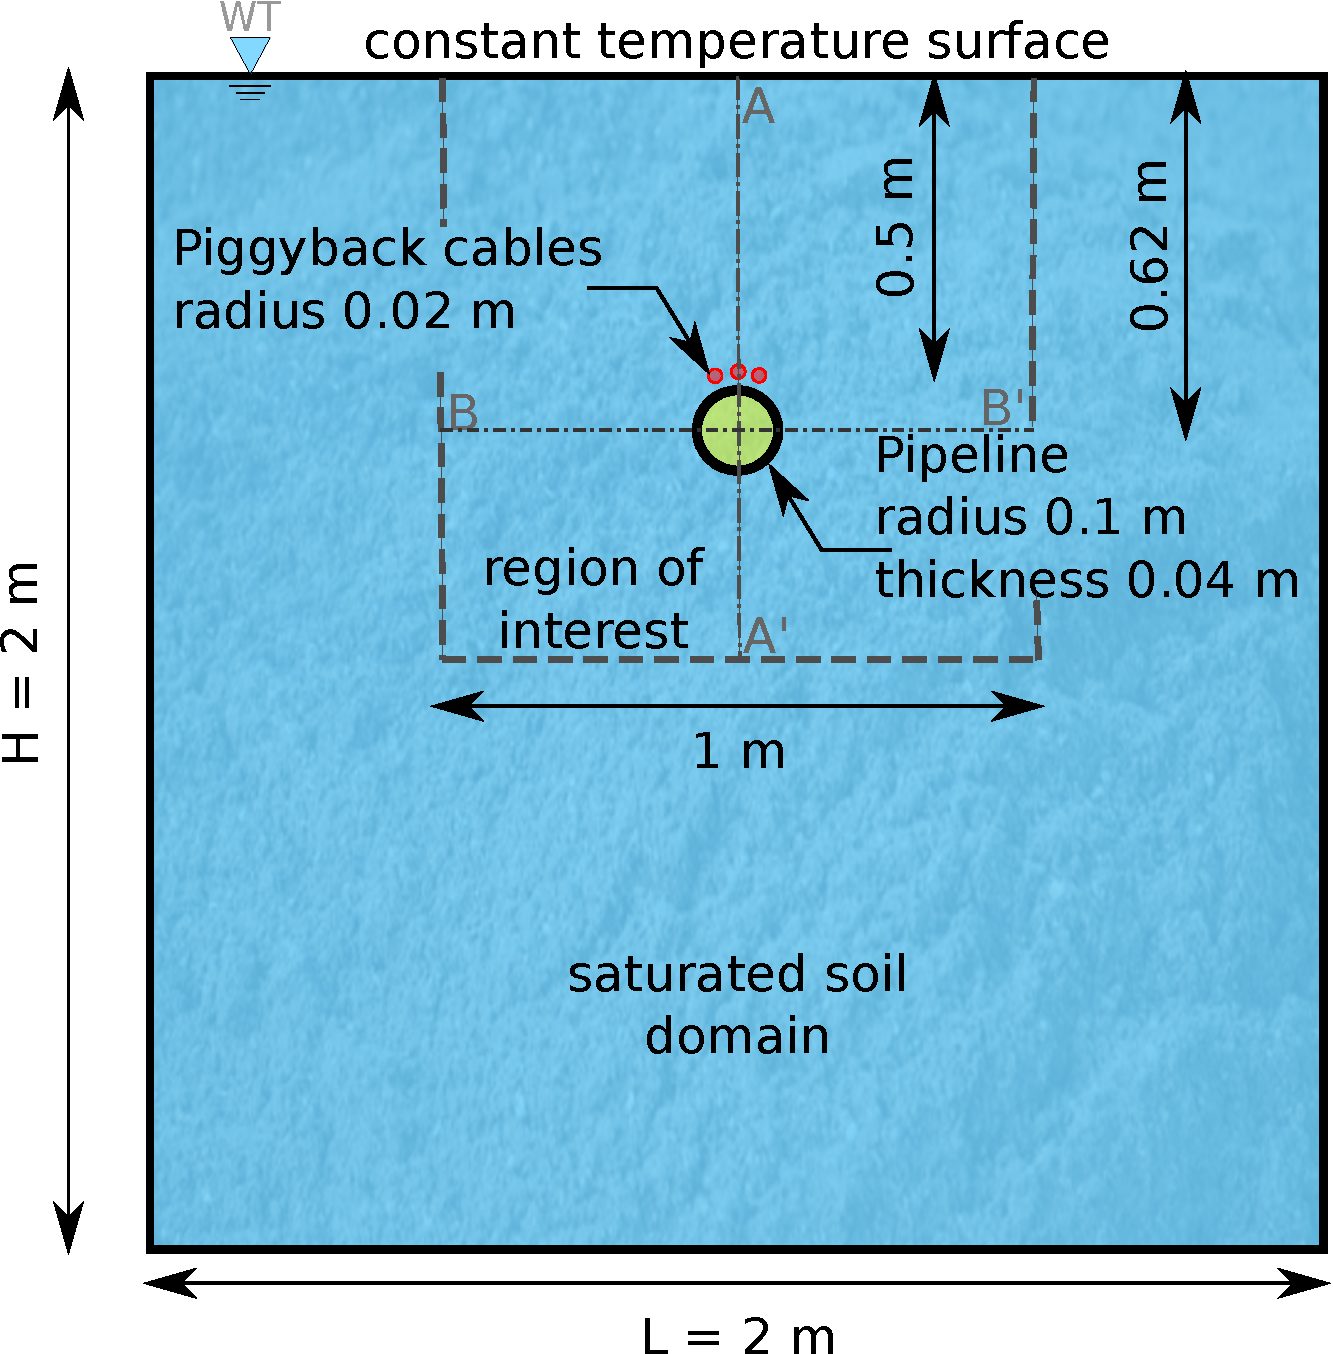
\includegraphics[width=\linewidth]{figs/model.pdf}
    \caption{Schematic of the simulation geometry (not to scale). A fine mesh size of 0.004 m was used to discretize the domain with 250,000 elements.}
    \label{fig:model}
\end{figure}

\subsection*{Material Properties}
We model the heat dissipation mechanisms for pipelines buried in different soil types from coarse-grained gravels and sands to fine-grained silts and clay. Soil permeability can vary over several orders of magnitude based on the porosity, mean grain radius, and grain size distribution. The semi-empirical Kozeny-Carman equation relates permeability to porosity and the mean grain size $d_m$:

\begin{equation}
k = \frac{1}{180} \frac{n^3}{(1-n^2)} d_m^2\,.
\end{equation}

Although clay is highly porous, the presence of an electrical double-layer reduces its effective porosity resulting in reduced permeability. We use the effective porosity only for the permeability calculation, while the soil density is calculated based on the actual porosity and assuming the pore space is fully saturated with water. The saturated unit weight of the soil is determined as:
\begin{equation}
 \gamma_{sat} = \frac{(G_s + e) \gamma_w}{1+e} \text{ and } n = \frac{e}{1+e}\,,   
\end{equation}
where $G_s$ is the specific gravity of solids, $e$ is the void ratio, $\gamma_w$ is the unit weight of water 9.81 $kN/m^3$, and $n$ is the soil porosity.~\Cref{tab:soil} presents the hydraulic and mechanical parameters of the soils used in this study. 

\begin{table}[]
\caption{Soil material properties}
\label{tab:soil}
\begin{tabular}{llcccc}
\toprule
\textbf{Properties}           &   \textbf{units}                      & \textbf{Gravel} & \textbf{Sand} & \textbf{Silt} & \textbf{Clay} \\
\midrule
Porosity ($n$)                  & -                       & 0.3 - 0.35      & 0.3 - 0.45    & 0.4 - 0.45    & 0.45 - 0.6    \\
Grain size ($d\_m$)             & mm                      & 7.5 - 20        & 0.1 - 2.5     & 0.025-0.07    & 0.002 - 0.02  \\
Specific gravity ($G_s$)         & -                       & 2.75            & 2.65          & 2.67          & 2.7           \\
Permeability ($k$)              & $m^2$    & 1E-7 - 1E-8     & 1E-9 - 1E-11  & 1E-12 - 1E-13 & 1E-13 - 1E-16 \\
Density ($\rho$) & $kg/m^3$ & 2100 - 2200     & 1870 - 2110   & 1880 - 1970   & 1650 - 1890  \\
\bottomrule
\end{tabular}
\end{table}

\Cref{tab:mat} presents the thermal properties of the fluid, soil, and cables. The bulk thermal conductivity and bulk specific heat of the porous media are calculated using simple arithmetic based on the volume fraction of fluid and solids:

\begin{align}
\lambda_b &= \lambda_s * (1 - n) + \lambda_f * n\,,\\
C_{p_b} &= C_{p_s} * (1 - n) + C_{p_f} * n\,.
\end{align}

The thermal diffusivity of the soil is:
\begin{equation}
\alpha_s = \lambda_b / (\rho * C_{p_b})\,.
\end{equation}

\begin{table}[]
\caption{Thermal properties of the fluid, soil, and the cables}
\label{tab:mat}
\centering
\begin{tabular}{ll}
\toprule
\textbf{Properties}                         & \textbf{Value}   \\
\midrule
\textbf{Fluid}                              &                  \\
Fluid density ($\rho_f$)                    & 1000 $kg/m^3$    \\
Specific heat of fluid ($Cp_f$)             & 4290 $J/kg-K$    \\
Thermal conductivity of fluid ($\lambda_f$) & 0.6 $W/m-K$      \\
Thermal diffusivity of fluid ($\alpha_f$)   & 1.39E-7 $m^2/s$  \\
Dynamic viscosity of fluid ($\mu$)          & 1E-3 $Pa-s$      \\
\textbf{Soil}                               &                  \\
Specific heat of soil ($C_{p_s}$)           & 8000 $J/kg-K$    \\
Thermal conductivity of soil ($\lambda_s$)  & 1.0 $W/m-K$      \\
\textbf{Pipe}                               &                  \\
Thermal diffusivity of pipe ($\alpha_p$)    & 1.172E-5 $m^2/s$ \\
\bottomrule
\end{tabular}
\end{table}

\pagebreak
%
\appendix
%
\section{Notation}
\label{app:notation}
The following symbols are used in this paper:
\nopagebreak
\par
\begin{tabular}{r  @{\hspace{1em}=\hspace{1em}}  l}
$D$                    & Depth of burial (m); \\
\end{tabular}

% \label{section:references}
\bibliography{ascexmpl-new}

\end{document}
